
% !TeX root = Report.tex
\phantomsection
\addcontentsline{toc}{subsection}{Lecture 3 - Iain Gavin \& Amazon Web Services: HAILO}
\subsect{Lecture 3 - Iain Gavin \& Amazon Web Services: HAILO}

%\inote{Spell checker is up the creek, all my sections need checking - Will do in Soton}





Amazon is, without any reasonable doubt, an established company. 
Founded by Jeff Bezos in 1994 as an online bookshop the company shipped their first book in July 1995~\cite{seattle}. 
Amazon now has three different parallel business interests. 
The original retail aspect, a 3$^{rd}$ party selling service via the website and Amazon Web Services (AWS).
AWS powers the other two aspects of the business by providing the IT infrastructure that enables such excellent customer service but also acts as an accelerator for other businesses by removing the requirement for on-premises IT solutions. 
They achieve this by maintaining large sever farms from which computing power can be \emph{rented} to facilitate the IT needs of a company. 
They also provide varying degrees of cloud based storage; subject to access latency.

AWS considers a typical split in effort toward a computing heavy business venture, with an on-premises IT solution, to be $30\%$ towards the actual business and $70\%$ towards IT overheads~\cite{gavin2014ams}. 
Their goal is to reverse this distribution by handling the IT infrastructure for the business. 
One such company that has succeeded using AWS is HAILO~\cite{gavin2014ams}. 
Launched in $2011$ with investments totalling over \$$80$ million (USD) from some well known sources such as Union Square Ventures, Accel Partners and Sir Richard Branson~\cite{hailo}.
The company maintains a smartphone app that links customers with the local taxi services however this idea is not unique. 
At the time there was already a large market for smartphone enabled cab rides so something else must have been their source of success~\cite{ventureBeat}. 
Market saturation and a software only product makes patenting redundant so it must have been down to the delivering and quality of the service that has made them a global success. 
Disassociating IT from the business using AWS may well have been a contributing factor to HAILO's ability to concentrate on product delivery.


The Amazon group as a whole is very technology driven, the founder filed the first two patents under ``Amazon.Com, Inc'' just before their first sale, and considers innovations as the best method to drive down the prices of the products they sell~\cite{bezos1998secure1,bezos1998secure2}. 
Reasoning behind this idea is shown in Figure~\ref{fig:ScaleInnovation}.
This cycle enables price reduction which naturally improves sales. 
The key step is providing the technology which can improve efficiency therefore staying ahead of competitors. 
Amazon keeps delivering the required technology, whilst patenting aggressively, and at the end of $2013$ created another media buzz by publishing a patent for ``anticipatory package shipping''~\cite{spiegel2013method}!



%\inote{Need to sexify}


\begin{figure}
	\centering
	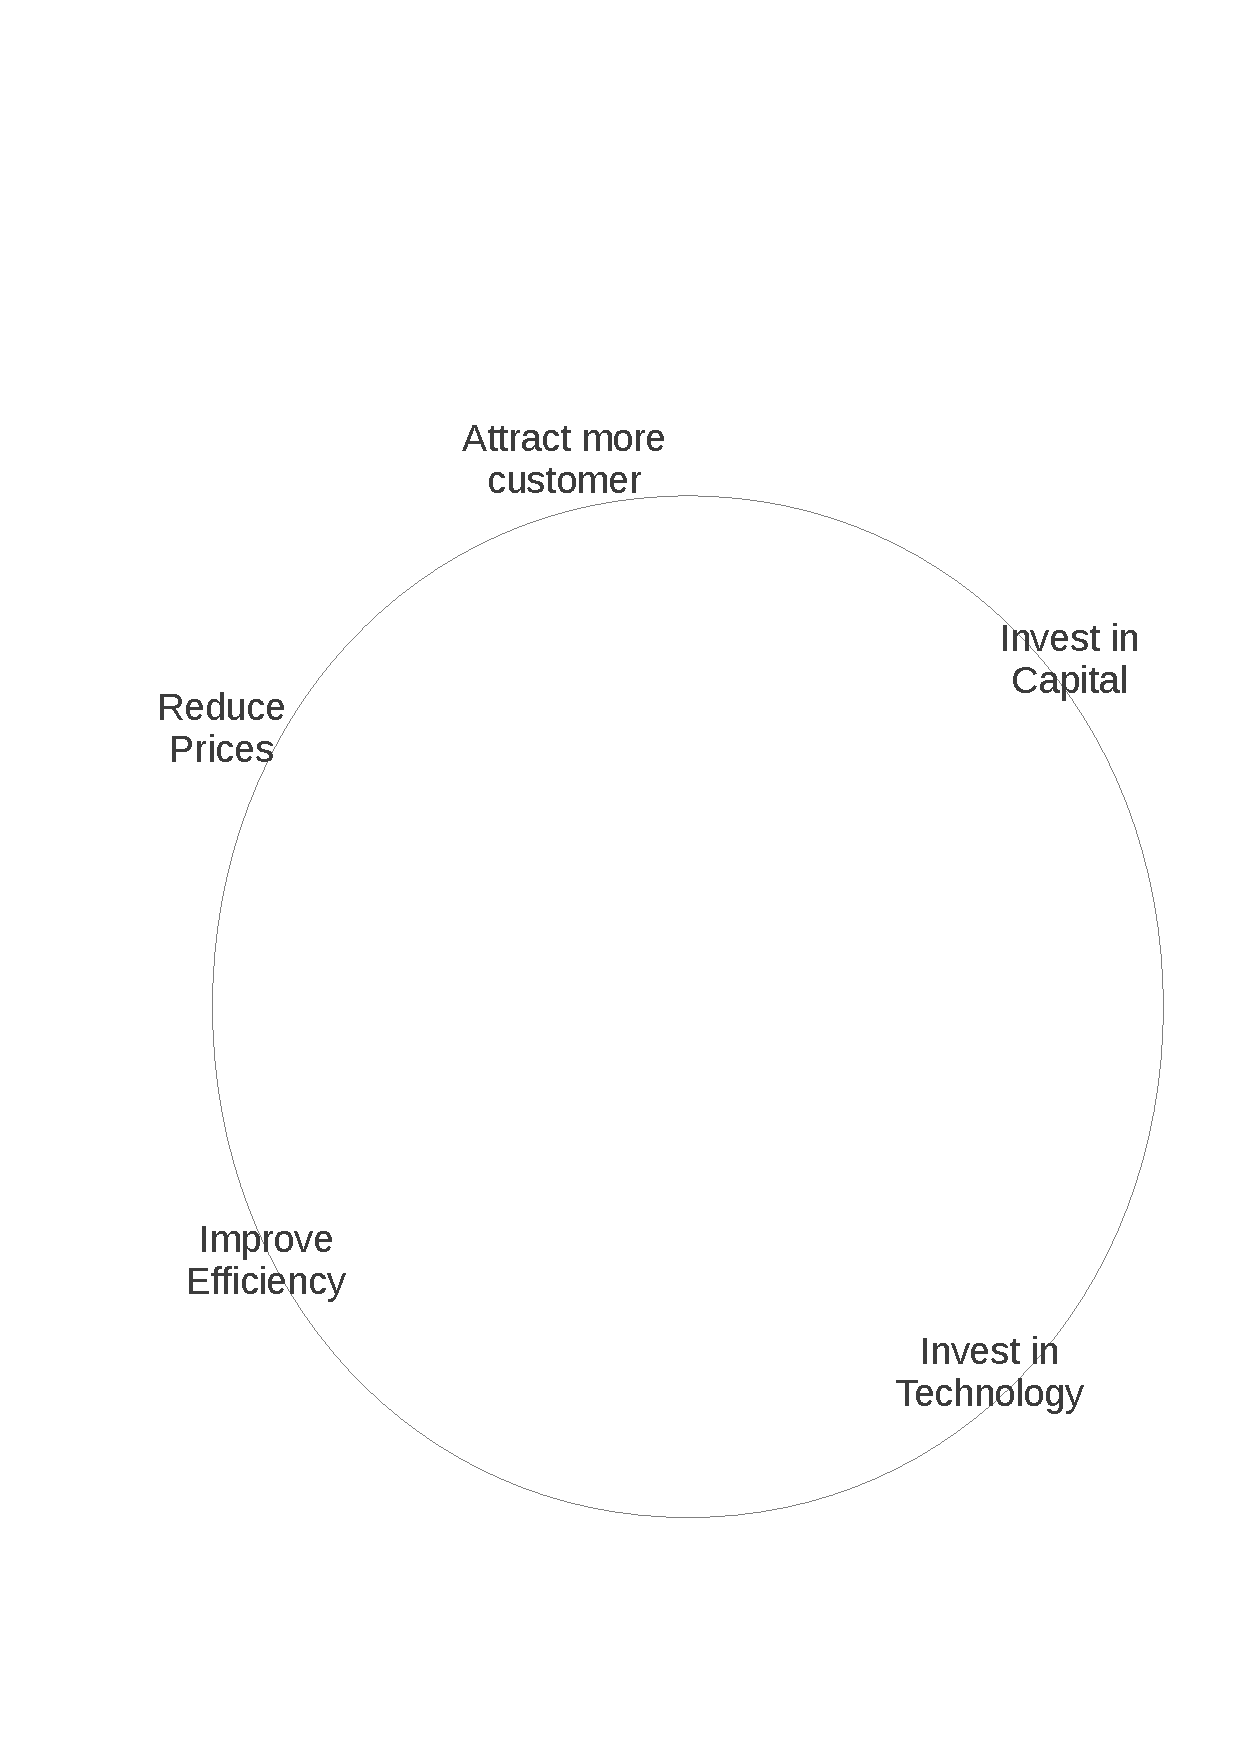
\includegraphics[width=0.4\textwidth]{./Figures/ScaleInnovation.pdf}
	\caption{Scale \& Innovation Drives Down Costs. Taken from~\cite{gavin2014ams}.}
	\label{fig:ScaleInnovation}
\end{figure}

